\documentclass[12pt,letterpaper,fleqn]{article}
\usepackage{fullpage}
\usepackage[top=2cm, bottom=4.5cm, left=2.5cm, right=2.5cm]{geometry}
\usepackage{amsmath,amsthm,amsfonts,amssymb,amscd}
\usepackage[utf8]{inputenc}
\usepackage{lastpage}
\usepackage{enumerate}
\usepackage{fancyhdr}
\usepackage{mathrsfs}
\usepackage{xcolor}
\usepackage{graphicx}
\usepackage{listings}
\usepackage{hyperref}
\usepackage{amsmath}
\usepackage{nccmath}

\newcommand{\R}{\mathbb{R}}
\newcommand{\Q}{\mathbb{Q}}

\hypersetup{%
  colorlinks=true,
  linkcolor=blue,
  linkbordercolor={0 0 1}
}
 
\renewcommand\lstlistingname{Algorithm}
\renewcommand\lstlistlistingname{Algorithms}
\def\lstlistingautorefname{Alg.}

\lstdefinestyle{Python}{
    language        = Python,
    frame           = lines, 
    basicstyle      = \footnotesize,
    keywordstyle    = \color{blue},
    stringstyle     = \color{green},
    commentstyle    = \color{red}\ttfamily
}

\setlength{\parindent}{0.0in}
\setlength{\parskip}{0.05in}

% Edit these as appropriate
\newcommand\course{Física - Frente 2}
\newcommand\hwnumber{1}                  % <-- homework number
\newcommand\NetIDa{netid19823}           % <-- NetID of person #1
\newcommand\NetIDb{netid12038}           % <-- NetID of person #2 (Comment this line out for problem sets)

\pagestyle{fancyplain}
\headheight 35pt
%\lhead{\NetIDa}
%\lhead{\NetIDa\\\NetIDb}                 % <-- Comment this line out for problem sets (make sure you are person #1)
\chead{\textbf{\Large Leis de Indução \hwnumber}}
\rhead{\course \\ Agosto/2019}
\lfoot{}
\cfoot{}
\rfoot{\small\thepage}
\headsep 1.5em

\begin{document}
    \begin{enumerate}
        \item \textbf{(UFSC)} - A figura abaixo representa um condutor colocado sob a ação de um campo magnético constante, com uma barra metálica apoiada sobre o condutor, deslocando-se com velocidade $\vec{V}$ 
        
        \begin{figure}[h]
            \centering
            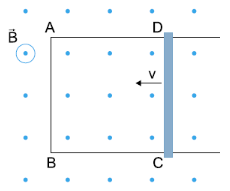
\includegraphics[width=0.7\textwidth]{ex_1.png}
        \end{figure}
        
        Dadas as alternativas:
        \begin{enumerate}
        \begin{enumerate}
            \item  O fluxo magnético no interior da espira ABCD está diminuindo, em módulo.
            \item A corrente induzida circula na espira no sentido anti-horário.
            \item A força que atua na barra é perpendicular à velocidade.
        \end{enumerate}
        \end{enumerate}
        
        Estão certas:
        \begin{enumerate}
            \item somente $i$
            \item somente $ii$
            \item somente $iii$
            \item duas delas
            \item todas
        \end{enumerate}
        
        \item \textbf{(UFRGS)} - A figura mostra três posições sucessivas de uma espira condutora que se desloca com velocidade constante numa região em que há um campo magnético uniforme, perpendicular à página e para dentro da página.
        
        \begin{figure}[h]
            \centering
            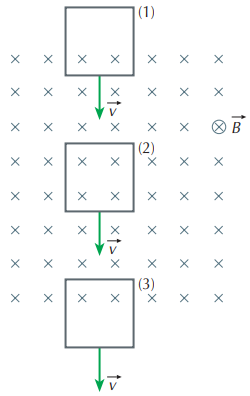
\includegraphics[width=0.3\textwidth]{ex_2.png}
        \end{figure}
        
        Selecione a alternativa que supre as omissões nas frases seguintes:
        
        \begin{enumerate}
        \begin{enumerate}
            \item  Na posição (1) a espira está penetrando na região onde existe o campo magnético e, consequentemente, está \underline{\hspace{2cm}} o fluxo magnético através da espira.
            \item  Na posição (2), não há \underline{\hspace{2cm}} na espira.
            \item Na posição (3), a corrente elétrica induzida na espira, em relação à corrente induzida na posição (1), tem sentido \underline{\hspace{2cm}}.
        \end{enumerate}
        \end{enumerate}
        
        
        \begin{enumerate}
            \item aumentando, fluxo, igual.
            \item diminuindo, corrente, contrário.
            \item diminuindo, fluxo, contrário.
            \item aumentando, corrente, contrário.
            \item diminuindo, fluxo, igual.
        \end{enumerate}
        
        \item \textbf{(UFMG)} - A figura a seguir mostra um imã próximo a um circuito constituído por uma bobina e um medidor sensível de corrente. Colocando-se a bobina e o ímã em determinados movimentos, o medidor poderá indicar passagem de corrente na bobina. Não haverá indicação de passagem de corrente pelo pelo medidor quando:
        
        \begin{figure}[h]
            \centering
            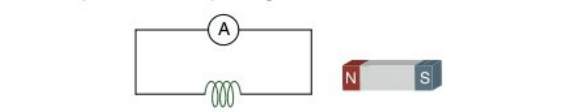
\includegraphics[width = 0.3\textwidth]{ex_3.png}
        \end{figure}
        
        \begin{enumerate}
            \item O imã e a bobina se movimentam, se aproximando-se;
            \item A bobina se aproxima do imã, que permanece parado;
            \item O imã se desloca para a direita e a bobina para esquerda; 
            \item O imã e a bobina se deslocam para a direita e ambos, com a mesma velocidade;
            \item O imã se aproxima da bobina e esta permanece parada.
        \end{enumerate}
        
        \item \textbf{(UNIFESP)} - A foto mostra uma lanterna sem pilhas, recentemente lançada no mercado. Ela funciona transformando em energia elétrica a energia cinética que lhe é fornecida pelo usuário – para isso ele deve agitá-la fortemente na direção do seu comprimento. Como o interior dessa lanterna é visível, pode-se ver como funciona: ao agitá-la, o usuário faz um ímã cilíndrico atravessar uma bobina para frente e para trás. O movimento do ímã através da bobina faz aparecer nela uma corrente induzida que percorre e acende a lâmpada.
        
        \begin{figure}[h]
            \centering
            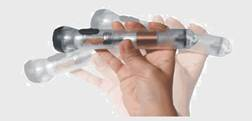
\includegraphics[width=0.7\textwidth]{ex_4.jpg}
        \end{figure}
        
        O princípio físico em que se baseia essa lanterna e a corrente induzida na bobina são, respectivamente:
        
        \begin{enumerate}
            \item Indução eletromagnética; corrente alternada.
            \item Indução eletromagnética; corrente contínua.
            \item Lei de Coulomb; corrente contínua.
            \item Lei de Coulomb; corrente alternada.
            \item Lei de Ampere; correntes alternada ou contínua podem ser induzidas.
        \end{enumerate}
        
        \item \textbf{(FUVEST)} -  Um anel de alumínio, suspenso por um fio isolante, oscila entre os pólos de um ímã, mantendo-se, inicialmente, no plano perpendicular ao eixo N - S e eqüidistante das faces polares. O anel oscila, entrando e saindo da região entre os polos, com uma certa amplitude.
        
        \begin{figure}[h]
            \centering
            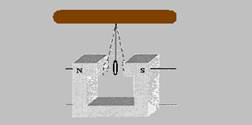
\includegraphics[width=0.7\textwidth]{ex_5.jpg}
        \end{figure}
        
        Nessas condições, sem levar em conta a resistência do ar e outras formas de atrito mecânico, pode-se afirmar que, com o passar do tempo:
        
        \begin{enumerate}
            \item A amplitude de oscilação do anel diminui. 
            \item A amplitude de oscilação do anel aumenta.
            \item A amplitude de oscilação do anel permanece constante. 
            \item O anel é atraído pelo polo Norte do ímã e lá permanece.
            \item O anel é atraído pelo polo Sul do ímã e lá permanece.
        \end{enumerate}
        
        \item \textbf{(UFMG - adaptado)} - Em uma aula, o Prof. Antônio apresenta uma montagem com dois anéis dependurados, como representado na figura anterior. Um dos anéis é de plástico - material isolante - e o outro é de cobre- material condutor. Inicialmente, o Prof. Antônio aproxima um imã, primeiro, do anel de plástico e, depois, do anel de cobre.
        
        \begin{figure}[h]
            \centering
            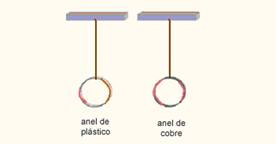
\includegraphics[width=0.7\textwidth]{ex_6.jpg}
        \end{figure}

Com base nessas informações, é CORRETO afirmar que:

\begin{enumerate}
    \item os dois anéis se aproximam do imã.
    \item o anel de plástico não se movimenta e o de cobre se afasta do imã.
    \item os dois anéis se afastam do imã.
    \item o anel de plástico não se movimenta e o de cobre se aproxima do imã
    \item Nenhuma das anteriores
\end{enumerate}

\item \textbf{(FEI)} - Em uma bobina, o fluxo magnético varia com o tempo, conforme o gráfico a seguir. Construa o gráfico da f.e.m ($\epsilon$) em função do tempo.

\begin{figure}[h]
    \centering
    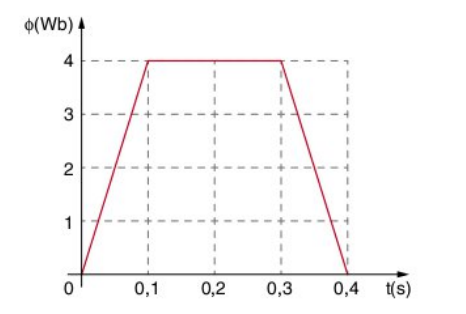
\includegraphics[width=0.7\textwidth]{ex_7.png}
\end{figure}

\item \textbf{(FAAP)} - Uma espira quadrada de lado igual a 8cm é perpendicular a um campo magnético, tal que a indução magnética vale $5.10^{-3}\: T$.

\begin{enumerate}
    \item Calcule o fluxo magnético ($\Phi$) que passa pela espira.
    \item Se o campo cai a 0 em 0,1 s, qual será a f.e.m média induzida na espira nesse intervalo de tempo?
\end{enumerate}

\item \textbf{(FAAP)} - Uma espira retangular de dimensões 30 cm por 10 cm, com resistência igual a 10 $\Omega$, move-se com velocidade de 5 cm/s na direção indicada na figura, perpendicularmente a um campo magnético uniforme de indução de 2T. Qual a intensidade da corrente elétrica na espira, 2s após a situação indicada na figura?

\textit{Dica: O exercício possui 2 partes: a parte de indução e a parte de cinemática. Resolva a parte de cinemática primeiro, considerando a figura como a situação t=0s. Se necessário, faça esboços. Lembre-se que a f.e.m é a tensão (U) aplicada à espira. Desconsidere qualquer força aplicada a espira.}

\begin{figure}[h]
    \centering
    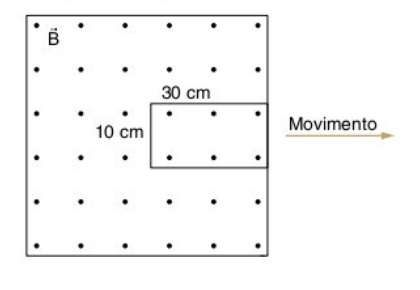
\includegraphics[width=0.7\textwidth]{ex_9.png}
\end{figure}

\pagebreak
\item \textbf{(ITA)} - Uma bobina circular de raio $R=1,0cm$ com 100 espiras de fio de cobre, colocada num campo de indução magnética constante e uniforme, tal que $B=1,2T$, está inicialmente numa posição em que o fluxo de $B$ através da bobina é máximo. Em seguida, num $\Delta t=1,5.10^{-2}s$, a bobina é girada para uma posição em que o fluxo de $B$ através dela é nulo. Qual é a força eletromotriz média induzida entre os terminais da bobina?

\item \textbf{(UERJ-RJ)} - O motorista dá partida no carro para iniciar sua viagem. O sistema de ignição do carro possui um conjunto de velas ligadas aos terminais de uma bobina de 30.000 espiras circulares. O diâmetro médio das espiras é igual a 4,0cm.  

Esse sistema, quando acionado, produz uma variação do campo magnético, , de $10^3T$ na bobina, sendo o campo perpendicular ao plano das espiras. Estabeleça o módulo da tensão resultante entre os terminais da bobina quando o sistema de ignição é acionado.

\textit{Considerar $\Delta t = 1\:s$}

\item \textbf{(FUVEST 2008)} - É possível acender um LED, movimentando-se uma barra com as mãos? 

Para verificar essa possibilidade, um jovem utiliza um condutor elétrico em forma de U, sobre o qual pode ser movimentada uma barra M, também condutora, entre as posições $X_1$ e $X_2$. Essa disposição delimita uma espira condutora, na qual é inserido o LED, cujas características são indicadas na tabela ao lado. 

Todo o conjunto é colocado em um campo magnético $B$ (perpendicular ao plano dessa folha e entrando nela), com intensidade de 1,1 T. O jovem, segurando em um puxador isolante, deve fazer a barra deslizar entre $X_1$ e $X_2$. 
\begin{figure}[h]
    \centering
    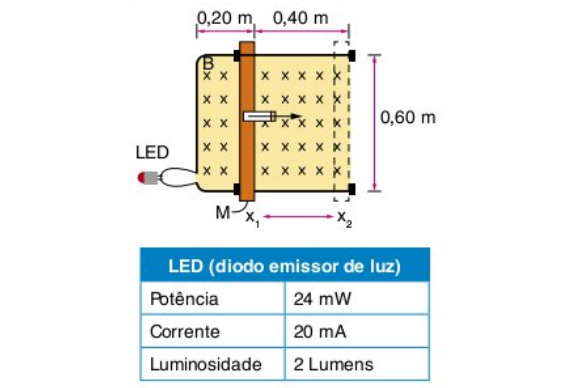
\includegraphics[width=0.7\textwidth]{ex_12.png}
\end{figure}

Para verificar em que condições o LED acenderia
durante o movimento, estime:

\begin{enumerate}
    \item  A tensão V, em volts, que deve ser produzida nos terminais do LED, para que ele acenda de acordo com suas especificações.
    \item  A variação $\Delta \Phi$ do fluxo do campo magnético através da espira, no movimento entre $X_1$ e $X_2$.
    \item O intervalo de tempo $\Delta t$, em s, durante o qual a barra deve ser deslocada entre as duas posições, com velocidade constante, para que o LED acenda.
\end{enumerate}

\item \textbf{(UFRGS)} - Um campo magnético cuja intensidade varia no tempo atravessa uma bobina de 100 espiras e de resistência elétrica desprezível. A esta bobina está conectada em série uma lâmpada cuja resistência é de 10,o $\Omega$ e que está dissipando 10,0 W. A variação temporal do fluxo magnético ($\Delta \Phi/ \Delta t$) através de cada espira é, em módulo, de:

\begin{enumerate}
    \item 0,01 Wb/s
    \item 0,10 Wb/s
    \item 1,0 Wb/s
    \item 10,0 Wb/s
    \item 100,0 Wb/s
\end{enumerate}
    \end{enumerate}
    
    \pagebreak
    \section*{GABARITO}
    
    \begin{enumerate}
        \item (d). O item iii está errado, pois a força atua paralelamente à velocidade, no caso no sentido oposto à velocidade.
        
        \item (d)
        \item (d)
        \item (a)
        \item (a)
        \item (b). O plástico não é material condutor, portanto ele não sofre indução magnética.
        \item 
        \item \begin{enumerate}
            \item $8\: cm \iff 0,08 \: m$
            
            $A= (0,08)^2 = 6,4.10^{-3}\:m^2$
            
            $\Phi = B.A.cos(\theta) \implies \Phi = 5.10^{-3}*6,4.10^{-3}$
            
            $\Phi = 3,2.10^{-5} \: Wb$
            
            \item $\epsilon = -\frac{\Delta \Phi}{\Delta t} \iff \epsilon= - \frac{\Phi_f - \Phi_i}{t_f-t_i}$
            
            $\epsilon = - \frac{0 - 3,2.10^{-5}}{0,1} \implies \epsilon = 3,2.10^{-6} \: V$
        \end{enumerate}
        
        \item Primeiro, vamos olhar a parte da cinemática, pois o campo magnético é uniforme, logo o valor dele é constante. Qualquer variação do fluxo magnético ($\Delta \Phi$), em que o fluxo é: $\Phi= B.A.cos(\theta)$, será pela variação da área ($\Delta A$), uma vez que a espira não gira (não se fala nada sobre isso no enunciado). 
     
        Então, vamos ver como a área varia no exercício. 
        
        Pela figura, vemos que com o passar do tempo, a largura do retângulo dentro da região vai diminuindo, então temos que achar qual é a largura do retângulo após 2 segundos: Para isso, vamos usar a equação do \textit{"sorvete"}.
        
        $S = S_0 + V.t \implies S = 30 - 5*2 \implies S = 20cm$
        
        Portanto, após 2s, a largura nova do retângulo é de 20cm. Com isso podemos calcular a área inicial e final do retângulo: (No SI)
        
        Inicial: $A_i = 0,1*0,3 = 3*10^{-2}\: m^2$
        
        Final: $A_f = 0,1*0,2 = 2*10^{-2}\: m^2$
        
        Ou seja, a variação de área entre o instante inicial e final é ($\Delta A$): 
        
        $\Delta A = A_f - A_i = -1*10^{-2} \: m^2$
        
        Como achamos como a área do retângulo nos 2 instantes, podemos calcular o fluxo nesses instantes e a variação do fluxo:
        
        $\Delta \Phi = \Phi_f - \Phi_i$
        
        $\Delta \Phi = B.A_f.cos(\theta) - B.A_i.cos(\theta)$, em que $A_f$ é a área final após 2s e $A_i$ é a área inicial dada na figura. Como o campo é perpendicular à espira, $\theta = 0$, logo $cos(\theta) = 1$. Na expressão acima $B$ é um fator comum, portanto:
        
        $\Delta \Phi = B.(A_f - A_i) = B.\Delta A$
        
        Substituindo os valores:
        
        $\Delta \Phi = 2*(-1.10^{-2}) \implies \Delta \Phi = -2.10^{-2} \: Wb$
        
        Usando a Lei de Faraday:
        
        $\epsilon = -\frac{\Delta \Phi}{\Delta t}$
        
        Lembrando que a espira se comporta como um circuito, e que a tensão (U) do circuito é a f.e.m ($\epsilon$), então:
        
        $\epsilon = R.i \implies \epsilon = 10.i$
        
        Substituindo de volta $\epsilon$ e colocando todos os dados obtidos na Lei de Faraday:
        
        $10.i = -\frac{-2.10^{-2}}{2} \implies i = 1.10^{-3} \: A$
        
        \item Fluxo máximo $\implies cos(\theta) =1$
        
        Fluxo mínimo $\implies cos(\theta) = 0$
        
        Como a bobina são 100 espiras, então o fluxo total da bobina ($\Delta \Phi_{total}$) será:
        
        $\Delta \Phi_{total} = 100*\Delta \Phi_{espira}$
        
        Com isso, lembrando que a espira é circular ($A=\pi R^2$), calculando o fluxo magnético quando ele é máximo (instante inicial):
        
        $\Phi_i = B.A.cos(\theta) \implies \Phi_i = 1,2*(\pi.(0,01)^2)*1$
        
        $\Phi_i = 1,2\pi*10^{-4} \: Wb$
        
        No instante final, o fluxo é nulo: $\Phi_f = 0$. Logo $\Delta \Phi_{espira} = -1,2\pi .10^{-4} \: Wb$
        
        Portanto: $\Delta \Phi_{total} = -1,2\pi . 10^{-2} \: Wb$
        
        Aplicando a Lei de Faraday:
        
        $\epsilon = - \frac{0 - 1,2\pi.10^{-2}}{1,5*10^{-2}} \implies \epsilon = 0.8\pi V$
        
        \item $d = 4,0 \: cm = 4.10^{-2} m \implies R = 2.10^{-2} m$
        
        A bobina é composta de 30000 espiras, logo:
        
        $\Delta \Phi_{total} = 30000*\Delta \Phi_{espira}$
        
        No acionamento do sistema, gera-se uma variação de campo magnético ($\Delta B$): $\Delta B = 10^3 \: T$
        
        Como o campo é perpendicular às espiras, então $cos(\theta) = 1$. Logo, a variação do fluxo magnético numa espira é:
        
        $\Delta \Phi_{espira} = \Delta B .A.cos(\theta)$
        
        A área da espira é: $A = \pi.R^2 = 4\pi.10^{-4}$
        
        Portanto: $\Delta \Phi_{espira} = 10^3.4\pi.10^{-4} \implies \Delta \Phi_{espira} = 0,4\pi \: Wb$
        
        Então, a f.e.m gerada na ignição é, pela Lei de Faraday:
        
        $\epsilon = - \frac{\Delta \Phi_{total}}{\Delta t} = - 30000 \frac{\Delta \Phi_{espira}}{\Delta t}$
        
        $\epsilon =  - 30000 \frac{0,4\pi}{1} \implies \epsilon = -12000\pi V$
        
        Como o exercício quer o módulo: $|\epsilon| = 12000\pi$
        
        \item
        \begin{enumerate}
            \item Usando a fórmula da potência elétrica:
            
            $P = U.i \iff 24.10^{-3} = 20.10^{-3}*V$
            
            $V = 1,2 V$
            
            \item A variação do fluxo magnético é devido a variação da área da espira, uma vez que o campo é constante. Como o campo é perpendicular à espira, $cos(\theta) =1$:
            
            $\Delta \Phi = B. \Delta A. cos(\theta) \implies \Delta \Phi = 1,1*0,4*0,6$
            
            $\Delta \Phi = 2,64.10^{-1} \: Wb$
            
            \item No nosso caso, a tensão (V) aplicada na espira é a f.e.m ($\epsilon$) induzida: $V = |\epsilon|$
            
            Logo: $V = \frac{\Delta \Phi}{\Delta t} \implies \Delta t = \frac{\Delta \Phi}{V}$
            
            $\Delta t = 2,64.10^{-1}/1,2 \implies  \Delta t = 0,22 \: s$
        \end{enumerate}
        
        \item (b). Lembrar que a potência elétrica pode ser escrita como: $P = \frac{V^2}{R}$, em que a tensão aplicada a bobina ($V$), nesse exercício, é a f.e.m ($\epsilon$). Como os dados do problema, descobre-se que $\epsilon = 10\:V$.
        
        Então é aplicar a Lei de Faraday: $\epsilon = -100 \frac{\Delta \Phi}{\Delta t}$
        
        Isolando o ${\Delta \Phi}{\Delta t}$, chega-se na resposta do item (b)
    \end{enumerate}
\end{document}
